\documentclass{article}
\usepackage[utf8]{inputenc}
\usepackage{caption}
\usepackage{subcaption}

\title{Practical Work 1}
\author {Hong Hanh}
\date{18 March 2019}

\usepackage{natbib}
\usepackage{graphicx}

\begin{document}

\maketitle

\begin{itemize}
    \item Install \textbf{traceroute} tool
    \item Check if \textbf{usth.edu.vn} is up or not with ping (5 times only)
    \begin{verbatim}
    root@Hanh:~# ping -c 5 usth.edu.vn
    PING usth.edu.vn (104.27.161.15) 56(84) bytes of data.
    64 bytes from 104.27.161.15: icmp_seq=1 ttl=56 time=158 ms
    64 bytes from 104.27.161.15: icmp_seq=2 ttl=56 time=145 ms
    64 bytes from 104.27.161.15: icmp_seq=3 ttl=56 time=244 ms
    64 bytes from 104.27.161.15: icmp_seq=4 ttl=56 time=806 ms
    64 bytes from 104.27.161.15: icmp_seq=5 ttl=56 time=366 ms

    --- usth.edu.vn ping statistics ---
    5 packets transmitted, 5 received, 0% packet loss, time 4183ms
    rtt min/avg/max/mdev = 145.377/344.320/806.927/244.391 ms
    \end{verbatim}
    % 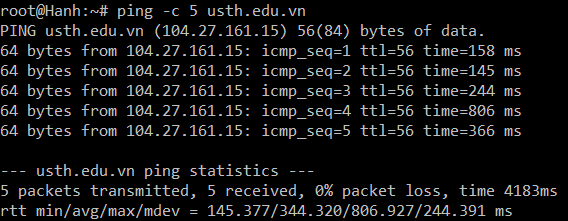
\includegraphics[scale=1.0]{ping.PNG}
    \item Use traceroute tool to find the route from your computer to
\textbf{usth.edu.vn}
    % 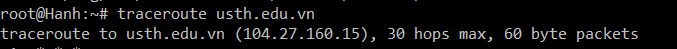
\includegraphics[scale=0.85]{traceroute.PNG}
    \begin{verbatim}
    root@Hanh:~# traceroute usth.edu.vn
    traceroute to usth.edu.vn (104.27.160.15), 30 hops max, 60 byte packets
        
    \end{verbatim}
\end{itemize}

\end{document}
